% Options for packages loaded elsewhere
\PassOptionsToPackage{unicode}{hyperref}
\PassOptionsToPackage{hyphens}{url}
%
\documentclass[
]{article}
\usepackage{lmodern}
\usepackage{amssymb,amsmath}
\usepackage{ifxetex,ifluatex}
\ifnum 0\ifxetex 1\fi\ifluatex 1\fi=0 % if pdftex
  \usepackage[T1]{fontenc}
  \usepackage[utf8]{inputenc}
  \usepackage{textcomp} % provide euro and other symbols
\else % if luatex or xetex
  \usepackage{unicode-math}
  \defaultfontfeatures{Scale=MatchLowercase}
  \defaultfontfeatures[\rmfamily]{Ligatures=TeX,Scale=1}
\fi
% Use upquote if available, for straight quotes in verbatim environments
\IfFileExists{upquote.sty}{\usepackage{upquote}}{}
\IfFileExists{microtype.sty}{% use microtype if available
  \usepackage[]{microtype}
  \UseMicrotypeSet[protrusion]{basicmath} % disable protrusion for tt fonts
}{}
\makeatletter
\@ifundefined{KOMAClassName}{% if non-KOMA class
  \IfFileExists{parskip.sty}{%
    \usepackage{parskip}
  }{% else
    \setlength{\parindent}{0pt}
    \setlength{\parskip}{6pt plus 2pt minus 1pt}}
}{% if KOMA class
  \KOMAoptions{parskip=half}}
\makeatother
\usepackage{xcolor}
\IfFileExists{xurl.sty}{\usepackage{xurl}}{} % add URL line breaks if available
\IfFileExists{bookmark.sty}{\usepackage{bookmark}}{\usepackage{hyperref}}
\hypersetup{
  hidelinks,
  pdfcreator={LaTeX via pandoc}}
\urlstyle{same} % disable monospaced font for URLs
\usepackage{graphicx}
\makeatletter
\def\maxwidth{\ifdim\Gin@nat@width>\linewidth\linewidth\else\Gin@nat@width\fi}
\def\maxheight{\ifdim\Gin@nat@height>\textheight\textheight\else\Gin@nat@height\fi}
\makeatother
% Scale images if necessary, so that they will not overflow the page
% margins by default, and it is still possible to overwrite the defaults
% using explicit options in \includegraphics[width, height, ...]{}
\setkeys{Gin}{width=\maxwidth,height=\maxheight,keepaspectratio}
% Set default figure placement to htbp
\makeatletter
\def\fps@figure{htbp}
\makeatother
\setlength{\emergencystretch}{3em} % prevent overfull lines
\providecommand{\tightlist}{%
  \setlength{\itemsep}{0pt}\setlength{\parskip}{0pt}}
\setcounter{secnumdepth}{-\maxdimen} % remove section numbering

\usepackage{ctex}

\title{12章实验}
\author{尹忠恩}
\date{\today}

\begin{document}

\maketitle

\newpage

\hypertarget{header-n0}{%
\section{chapter12}\label{header-n0}}

\hypertarget{header-n2}{%
\subsection{代码}\label{header-n2}}

\begin{verbatim}
assume cs:code

code segment
start:


    call transfer

    ;demo
    mov ax,1000h
    mov bh,1
    div bh

    mov ax,4c00h
    int 21h
;=================================================
transfer:
    ;mov d0
    mov ax,cs
    mov ds,ax
    mov si,offset do0

    mov ax,0
    mov es,ax
    mov di,200h

    mov cx,offset do0_end - offset do0

    cld
    rep movsb

    ;set int table
    mov ax,0
    mov es,ax
    mov word ptr es:[0*4],200h
    mov word ptr es:[0*4+2],0

    ret

;===========================================
do0:
    jmp short do0_bg
    db 'divide error!'
do0_bg:

    mov ax,cs
    mov ds,cx
    mov si,202h

    mov ax,0b800h
    mov es,ax
    mov di,160*12+2*34

    mov cx,13
    s:
        mov al,ds:[si]
        mov ah,2
        mov es:[di],ax
        inc si
        add di,2
        loop s

    mov ax,4c00h
    int 21h

do0_end:
    nop

code ends
end start
\end{verbatim}

\hypertarget{header-n6}{%
\subsection{截屏}\label{header-n6}}

\begin{figure}
\centering
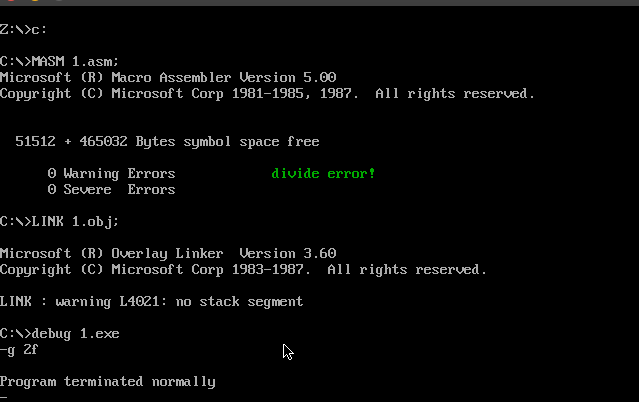
\includegraphics{/home/shenxin/workspace/ASM/实验文档/chapter12/Untitled.assets/Screenshot_20200319_132229.png}
\caption{}
\end{figure}

\end{document}
